\section{Simulation Results}
\label{sec:simulation_results}

\begin{figure*}[!t]
	\centering
	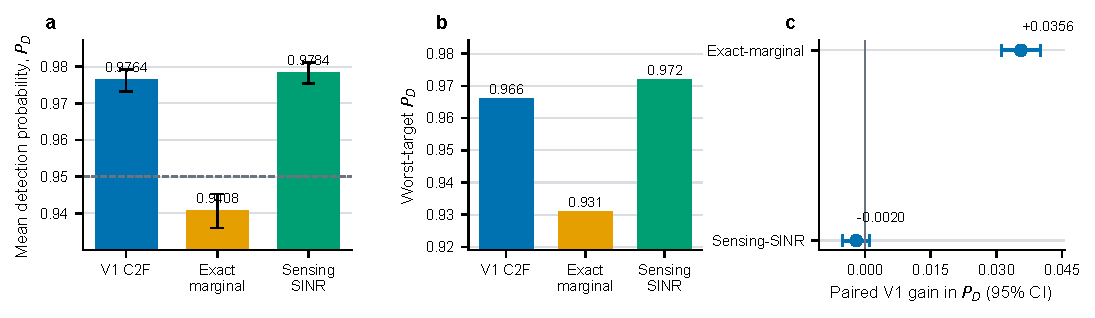
\includegraphics[width=0.98\textwidth]{figs/fig2_v1_main_comparison.pdf}
	\caption{Confirmatory MC=1000 comparison under identical per-trial resources.
	(a) Mean detection probability with 95\% Wilson intervals; the dashed line
	marks 0.95. (b) Worst-target detection probability. (c) Paired V1-minus-
	baseline differences with 95\% confidence intervals.}
	\label{fig:v1_main}
\end{figure*}

\begin{figure*}[!t]
	\centering
	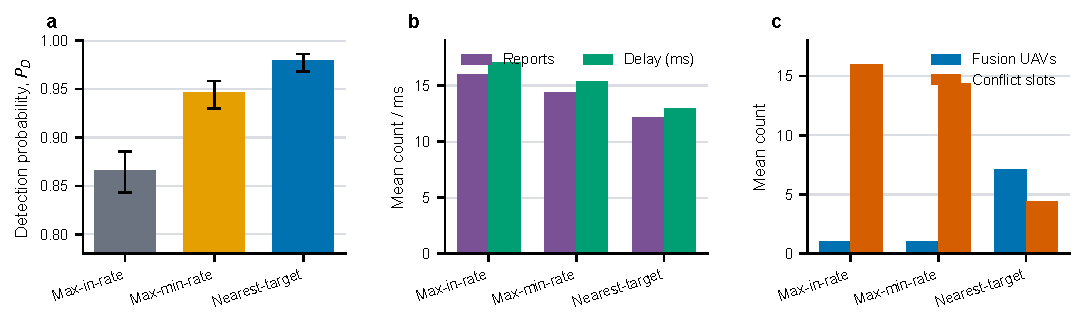
\includegraphics[width=0.98\textwidth]{figs/fig3_v1_fusion_ablation.pdf}
	\caption{Fusion-rule mechanism ablation (MC=100 per rule) with the inner
	adaptive C2F selector fixed. (a) Detection probability and 95\% intervals.
	(b) Selected reports and measured serial delay. (c) Number of assigned fusion
	UAVs and conflict-graph slots. The slot count diagnoses parallelization
	potential; it is not an achieved latency.}
	\label{fig:fusion_ablation}
\end{figure*}

\begin{figure*}[!t]
	\centering
	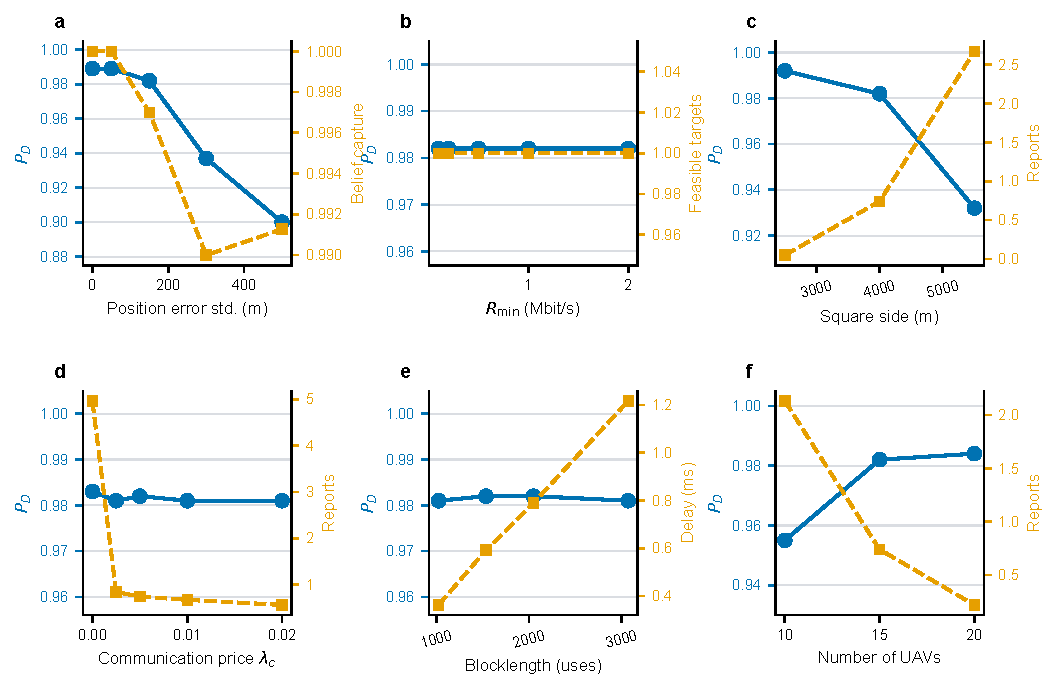
\includegraphics[width=0.98\textwidth]{figs/fig4_v1_operating_envelope.pdf}
	\caption{Exploratory V1 operating envelope (MC=100 per condition). Blue circles
	show $P_D$; orange squares show the named secondary metric. (a) Position-belief
	error, (b) minimum reporting rate, (c) deployment side length, (d)
	communication price, (e) blocklength, and (f) UAV fleet size.}
	\label{fig:operating_envelope}
\end{figure*}

\subsection{Protocol and Nominal Configuration}

We evaluate prior-assisted confirmation in a $4000\,\mathrm{m}\times
4000\,\mathrm{m}$ region with $M=15$ UAVs and $Q=10$ targets. Table~
\ref{tab:simulation_parameters} lists the released V1 configuration. All main
methods use the same paired geometries, detector randomness, feasible graph,
and per-trial number of selected reports. The confirmatory comparison uses 1000
Monte-Carlo trials. Fusion and operating-envelope sweeps use 100 trials per
condition with seed 2026 and are therefore diagnostic rather than substitutes
for the main evidence.

\begin{table}[!t]
	\centering
	\caption{Target-local fusion V1 simulation parameters}
	\label{tab:simulation_parameters}
	\footnotesize
	\setlength{\tabcolsep}{3pt}
	\begin{tabular}{@{}p{0.43\linewidth}p{0.51\linewidth}@{}}
		\toprule
		Parameter & Value \\
		\midrule
		UAVs / targets & $M=15$, $Q=10$ \\
		Area / communication range & $4000^2~\mathrm{m}^2$, $d_{\max}=2500~\mathrm m$ \\
		UAV / target speed & $30$--$60$ / $50$--$90~\mathrm{m/s}$ \\
		Carrier / DD grid & $5.9~\mathrm{GHz}$, $N=L=64$, $\Delta f=30~\mathrm{kHz}$ \\
		Power split / transmit power & $\rho=0.8$, $P_i=1~\mathrm W$ \\
		Rate threshold / false alarm & $R_{\min}=0.2~\mathrm{Mbit/s}$, $P_{\mathrm{FA}}=0.05$ \\
		Report / blocklength & 640 bits, $n=2048$ channel uses \\
		Predicted belief & $\sigma_p=150~\mathrm m$, $\sigma_v=15~\mathrm{m/s}$ \\
		Selection & $D_{\min}=3$, $\lambda_c=0.005$, $L_{\max}=6$, $L_{\mathrm{tot}}=60$ \\
		Fusion / reporting & nearest predicted target / serial orthogonal MAC \\
		C2F refinement & $W=1$, adaptive frontier, detector-aligned replay \\
		Main / sweep trials & 1000 / 100 per condition \\
		\bottomrule
	\end{tabular}
\end{table}

\subsection{Confirmatory Main Comparison}

Figure~\ref{fig:v1_main} compares target-local adaptive C2F with two strong
resource-matched rules. Exact-marginal greedy uses the same fair utility but no
C2F detector-aligned replay; Sensing-SINR ranks nominal sensing strength. V1
attains $P_D=0.9734$ (95\% CI: $[0.9701,0.9764]$), versus 0.9667 for
exact-marginal greedy and 0.9649 for Sensing-SINR. Its worst-target detection
probability is 0.968, compared with 0.957 and 0.953. The paired gains are
$+0.0067$ (95\% CI: $[0.0041,0.0093]$) and $+0.0085$
($[0.0061,0.0109]$), respectively; both interval lower bounds are positive.
The empirical active-target and system-wide false-alarm probabilities are
0.0498 and 0.0495, consistent with the designed value 0.05.

Resource matching is exact: each method selects 11.993 reports on average,
corresponding to 7.676~kbit and 12.793~ms of serial reporting. Thus, the main
detection gain is not purchased with more reports. The adaptive C2F stage
evaluates 117.7 fine DD neighborhoods instead of 509.3 for exhaustive local
refinement, reducing fine evaluations by 76.9\%. These results support the V1
system as a stable nominal point; they do not isolate fusion placement because
all three main methods already use the target-local graph.

\subsection{Why Target-Local Fusion Helps}

Figure~\ref{fig:fusion_ablation} changes only the fusion destination rule. The
target-agnostic max-in-rate rule gives $P_D=0.866$, worst-target $P_D=0.800$,
15.99 reports, and 17.056~ms. A max-min-rate alternative improves these values
to 0.946, 0.930, 14.36, and 15.317~ms. Nearest-target fusion reaches 0.979 and
0.960 with only 12.16 reports and 12.971~ms. Because the two-stage screening,
greedy objective, packets, and caps are unchanged, this ablation supports the
mechanism in \eqref{eq:nearest_target_fusion}: fusion placement changes the
reliable reporting-edge set seen by the selector.

The reporting structure explains the difference. Max-in-rate and max-min-rate
assign all ten targets to one fusion UAV on average. Nearest-target assigns
them across 7.13 UAVs and lowers the mean conflict-graph requirement from
15.99/14.36 to 4.40 slots. If reports in nonconflicting edges could be sent
simultaneously without bandwidth sharing, additional interference, or a changed
finite-blocklength model, 4.40 slots would correspond to a 4.693~ms lower
bound. V1 does not implement this scheduler, so its reported latency remains
the measured serial value 12.971~ms.

\subsection{Operating Envelope and Design Choices}

Figure~\ref{fig:operating_envelope} summarizes six controlled scans. First,
V1 remains near $P_D=0.98$ for position-error standard deviations up to 150~m,
then decreases to 0.960 at 300~m and 0.918 at 500~m. Belief capture remains
0.9868 even at 500~m; the degradation is therefore more consistent with
prediction-induced fusion and link mismatch than with DD-gate misses alone.
Second, $R_{\min}\le0.5$~Mbit/s is inactive at this nominal geometry. At
2~Mbit/s, only 94\% of targets retain feasible candidates and $P_D$ falls to
0.901; the lower report count is candidate starvation, not improved efficiency.

Topology is the next boundary. Increasing the square side from 2500 to 5500~m
changes $P_D$ from 0.992 to 0.913 and reports from 10.19 to 15.87. Increasing
the fleet from 10 to 20 UAVs at $Q=10$ changes $P_D$ from 0.941 to 0.987 while
reducing reports from 15.01 to 10.94. These scans vary density implicitly and
must not be combined into an independent density effect.

The communication price exhibits a broad plateau. Setting $\lambda_c=0$
requires 16.29 reports at $P_D=0.978$, whereas $\lambda_c=0.005$ uses 12.16
reports at $P_D=0.979$. Values from 0.0025 to 0.01 have overlapping MC=100
uncertainty, so 0.005 is treated as a stable engineering point rather than a
statistically unique optimum. Finally, 2048 channel uses yields
$P_D=0.979$ and 12.971~ms. The 1536-use setting is a promising lower-latency
candidate (0.977, 9.880~ms), while 3072 uses is dominated in this scan (0.975,
19.136~ms). A paired high-MC comparison is required before promoting the
1536-use setting to a new release.

All figures are generated directly from the released CSV/JSON records. The
resolved V1 configuration, source-data index, and plotting command accompany
the manuscript, preventing exploratory and confirmatory results from being
silently mixed.
